\section{Biological Background}

\begin{figure}[h]
  \centering
	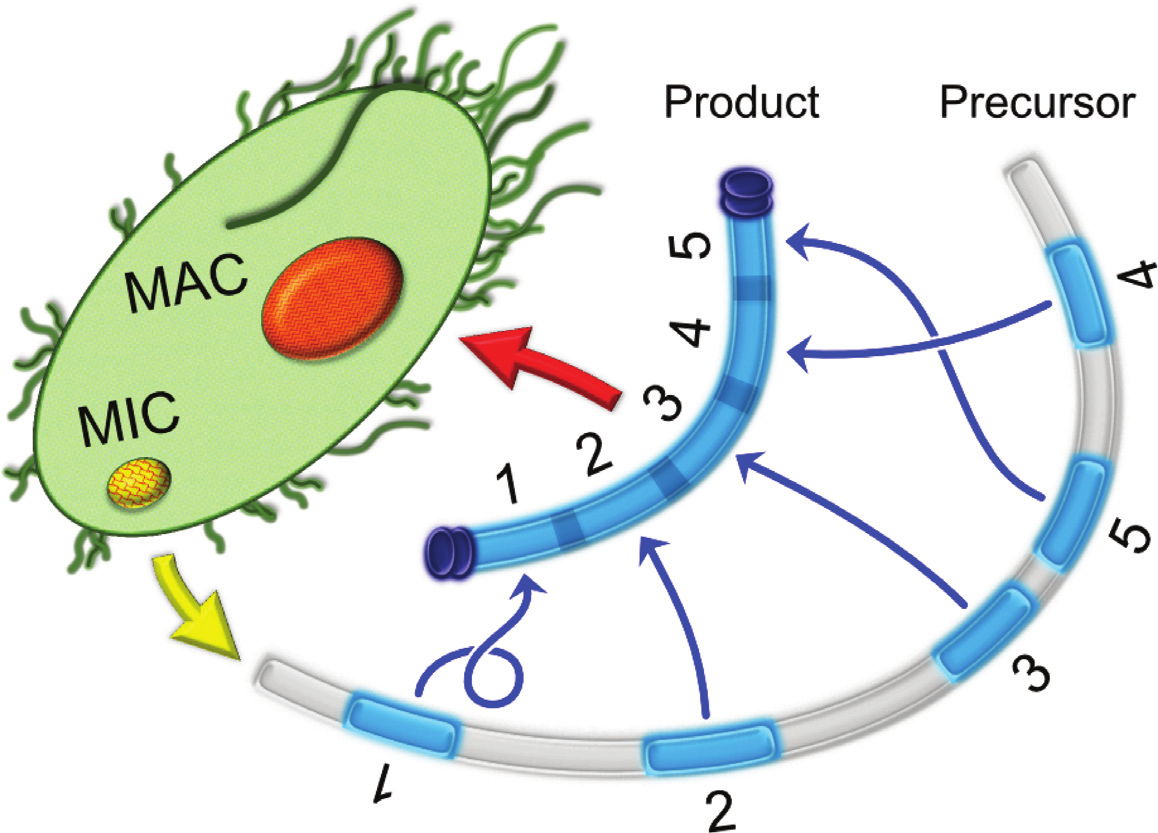
\includegraphics[width=250px]{0}
  \caption{In the somatic macronucleus (MAC), chromosomes assemble from precursor MDS building blocks (blue), which may be scrambled in some species. In the germline micronucleus (MIC), the Macronuclear Destined Sequences (MDSs) for all somatic chromosomes are dispersed over the long chromosome, and interrupted by Internally-Eliminated Sequences (IESs) and other noncoding DNA (gray). In some cases, an MDS may appear in a permuted order, or inverted.\cite{mdsiesdb}.
}
\end{figure}

Ciliated protists (microbial eukaryotes using cilia for locomotion) exhibit nuclear dimorphism through the presence of separate germline and somatic nuclei. The somatic macronucleus (MAC) provides templates for the transcription of all genes required for asexual growth while the germline micronucleus (MIC) is used for the exchange of meiotic products during sexual reproduction \cite{mdsiesdb}.

Several species of ciliates, such as Stylonychia or Oxytricha, go through extensive gene rearrangement while differentiating somatic macronuclei from germline micronuclei: an extensive fragmentation, elimination and sometimes broader rearrangement of the germline DNA, coupled to DNA amplification and telomere addition \cite{ciliatedDNA} forms the somatic macronuclei.



The ciliate Oxytricha is a microbial eukaryote with two genomes, one of which experiences
extensive genome remodeling during development. Each round of conjugation initiates a cascade
of events that construct a transcriptionally active somatic genome from a scrambled germline
genome, with considerable help from both long and small noncoding RNAs.
\section{Biological Motivation}
\cite{ANGELESKA20093020}

\section{Formalisation}

\begin{figure}[h]
  \centering
    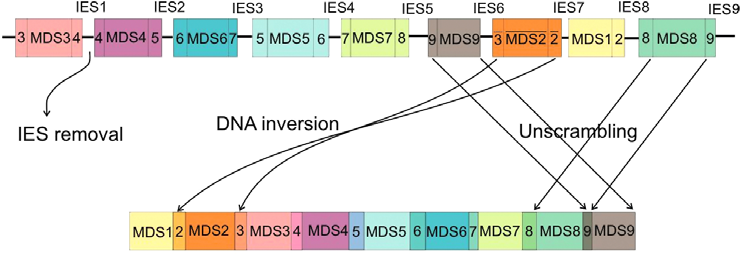
\includegraphics[width=\textwidth]{1}
  \caption{Schematic representation of the scrambled Actin I micronuclear germline gene in Oxytricha nova (top) and the correctly assembled macronuclear gene (bottom). Each block represents an MDS, and each line between blocks is an IES. The numbers at the beginning and at the end of each segment represent the pointer sequences. Note that MDS3· · ·MDS8 require permutation and inversion to assemble into the orthodox, linear order MDS1· · ·MDS9 in the macronucleus. The bars above MDS2 and its pointers indicate that this block is inverted relative to the others, i.e., this sequence is the Watson - Crick reverse complement of the version in the macronucleus; from\cite{prescottgreslin}.}

\end{figure}

\section{Existent Approaches/Solutions}

\section{ILP formulation}